\documentclass[a4paper,11pt]{article}
\usepackage[utf8]{inputenc}
\usepackage{latexsym}
\usepackage[empty]{fullpage}
\usepackage{titlesec}
\usepackage{marvosym}
\usepackage[usenames,dvipsnames]{color}
\usepackage{verbatim}
\usepackage{enumitem}
\usepackage[hidelinks]{hyperref}
\usepackage{palatino}
\usepackage{tikz}
\usepackage{tabularx}
\usepackage{fontawesome}
\input{glyphtounicode}

% Page setup
\addtolength{\oddsidemargin}{-1cm}
\addtolength{\evensidemargin}{-1cm}
\addtolength{\textwidth}{2cm}
\addtolength{\topmargin}{-1cm}
\addtolength{\textheight}{2cm}
\urlstyle{same}
\raggedbottom
\raggedright
\setlength{\tabcolsep}{0cm}
\pdfgentounicode=1

% Sections formatting
\titleformat{\section}{
  \vspace{-4pt}\scshape\raggedright\large
}{}{0em}{}[\color{black}\titlerule \vspace{-5pt}]

% Custom commands
\newcommand{\CVItem}[1]{
  \item\small{#1 \vspace{-2pt}}
}

\newcommand{\CVSubheading}[4]{
  \vspace{-2pt}\item
    \begin{tabular*}{0.97\textwidth}[t]{l@{\extracolsep{\fill}}r}
      \textbf{#1} & #2 \\
      \small#3 & \small #4 \\
    \end{tabular*}\vspace{-7pt}
}

\newcommand{\CVSubSubheading}[2]{
  \item
    \begin{tabular*}{0.97\textwidth}{l@{\extracolsep{\fill}}r}
      \text{\small#1} & \text{\small #2} \\
    \end{tabular*}\vspace{-7pt}
}

\newcommand{\CVSubItem}[1]{\CVItem{#1}\vspace{-4pt}}

\newcommand{\CVSubHeadingListStart}{\begin{itemize}[leftmargin=0.5cm, label={}]}
\newcommand{\CVSubHeadingListEnd}{\end{itemize}}
\newcommand{\CVItemListStart}{\begin{itemize}}
\newcommand{\CVItemListEnd}{\end{itemize}\vspace{-5pt}}

\begin{document}

% -----HEADING-------------------------------------------------------
\begin{minipage}[c]{0.25\textwidth}
  \begin{center}
    \begin{tikzpicture}
      \clip (0,0) circle (1.75cm);
      \node at (0,0) {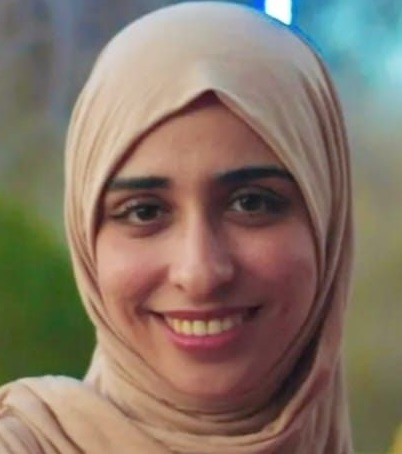
\includegraphics[width=3.5cm]{img}};
    \end{tikzpicture}
  \end{center}
\end{minipage}
\begin{minipage}[c]{0.7\textwidth}
  {\huge \textbf{Oumayma Metoui}}\\[4pt]
  {\large \textbf{Senior Fullstack JS}}\\[8pt]

  \small{
  Ingénieure Fullstack avec 7+ ans d'expérience dans les systèmes industriels (MES), l'architecture temps réel et les applications web critiques. Spécialisée dans les environnements de production avec forte volumétrie de données.
  }\\[12pt]

  \small
  Téléphone : +216 55 158 591 \hspace{15pt} \\
  Email : \href{mailto:oumayma.metoui@gmail.com} {oumayma.metoui@gmail.com} \\
  LinkedIn : \href{https://linkedin.com/in/oumayma-metoui-9506412a5}{linkedin.com/in/oumayma-metoui-9506412a5} \hspace{15pt} \\
  GitHub : \href{https://github.com/oumayma26} {github.com/oumayma26} \\
  Portfolio : \href{https://oumayma-portfolio-five.vercel.app/}{oumayma-portfolio-five.vercel.app}
\end{minipage}


% -----EXPERIENCE-------------------------------------------------------
\section{Expérience Professionnelle}
  \CVSubHeadingListStart
    \CVSubheading
      {Ingénieure FullStack JS -- Lead Technique}{Septembre 2018 -- Avril 2025}
      {Marabout Technology}{Tunis, Tunisie}
      \CVItemListStart
        \CVItem{\textbf{Architecture \& Performance :} Conception d'une architecture Angular modulaire (lazy loading, modules métier séparés) réduisant le temps d'ajout de fonctionnalités de 30\%.}
        \CVItem{\textbf{Système MES Industriel :} Conception et évolution d'un système MES (Manufacturing Execution System) pour le suivi temps réel de la production textile, réduisant les erreurs de reporting de 40\%.}
        \CVItem{\textbf{Backend \& APIs :} Développement d'APIs REST sécurisées (JWT, rate limiting) et intégration RabbitMQ pour le traitement asynchrone de données de production.}
        \CVItem{\textbf{Temps Réel :} Implémentation WebSocket (Socket.IO) pour le monitoring temps réel des lignes de production et alertes automatiques.}
        \CVItem{\textbf{Base de Données :} Optimisation des requêtes PostgreSQL critiques (indexation, requêtes matérialisées) réduisant le temps de réponse des dashboards de 60\%.}
        \CVItem{\textbf{Déploiement \& DevOps :} Gestion des déploiements backend avec PM2, configuration Apache pour le frontend, conteneurisation Docker des services.}
        \CVItem{\textbf{Stack :} Angular 18, Node.js, NestJS, PostgreSQL, RabbitMQ, Redis, Socket.IO, Docker, PM2, Apache.}
      \CVItemListEnd

    \CVSubheading
      {Ingénieure Java Spring / Angular}{Octobre 2017 -- Août 2018}
      {Solution Group}{Tunis, Tunisie}
      \CVItemListStart
        \CVItem{Développement d'une application de gestion d'assurance (Spring Boot, Angular) avec module de souscription en ligne.}
        \CVItem{Création d'un site web responsive avec design moderne et accessibilité.}
        \CVItem{Développement d'une application PHP pour la gestion des factures et automatisation des processus financiers.}
      \CVItemListEnd

    \CVSubheading
      {Stagiaire -- Développeuse Spring / Angular}{Octobre 2016 -- Décembre 2016}
      {Centre National de l'Informatique (CNI)}{Tunis, Tunisie}
      \CVItemListStart
        \CVItem{PFE : Conception et développement d'une application Spring de suivi des paies (Spring Boot, Spring Security, Spring Data, AngularJS, Bootstrap).}
      \CVItemListEnd

    \CVSubheading
      {Stagiaire -- Développeuse Java}{Février 2014 -- Mai 2014}
      {Caisse Nationale de Sécurité Sociale}{Tunis, Tunisie}
      \CVItemListStart
        \CVItem{PFE : Conception et développement d'une application de gestion de formation (Java EE, Hibernate, MySQL).}
      \CVItemListEnd
  \CVSubHeadingListEnd


% -----EDUCATION--------------------------------------------------------
\section{Formation}
  \CVSubHeadingListStart
    \CVSubheading
      {Mastère Professionnel -- Ingénierie des Systèmes d'Information}{2015 -- 2017}
      {École Nationale d'Ingénieurs de Carthage (ENICar)}{Tunis, Tunisie}
    \CVSubheading
      {Licence en Informatique -- Systèmes Informatique et Logiciel}{2011 -- 2013}
      {École Nationale d'Ingénieurs de Carthage (ENICar)}{Tunis, Tunisie}
  \CVSubHeadingListEnd

% -----SKILLS----------------------------------------------------------
\section{Compétences Techniques}
 \begin{itemize}[leftmargin=0.5cm, label={}]
    \small{
     \item \textbf{Frontend :} Angular (18+), React, TypeScript, RxJS, Angular Material, HTML5, CSS3, Tailwind CSS, Bootstrap
     \item \textbf{Backend :} Node.js (Express.js, NestJS), RESTful APIs, GraphQL, Socket.IO, WebSocket
     \item \textbf{Base de Données :} PostgreSQL, MySQL, MongoDB, Redis (cache, sessions)
     \item \textbf{Message Broker \& Temps Réel :} RabbitMQ, Apache Kafka, Socket.IO, WebSocket
     \item \textbf{DevOps & Outils :} Docker, Docker Compose, PM2, Apache, Nginx, Git, GitHub Actions
     \item \textbf{Méthodologies :} Agile (Scrum, Kanban)
    }
 \end{itemize}

% -----CERTIFICATIONS----------------------------------------------------------
\section{Certifications}
\begin{itemize}[leftmargin=0.5cm]
  \item \textbf{React de A à Z (Hooks, Redux)} -- Udemy \\
  \href{https://www.udemy.com/certificate/UC-96bada52-dbe8-46e7-9bc3-90d3e0377070/}{\textit{Voir la certification en ligne}}
\end{itemize}

% -----LANGUES---------------------------------------------------------
\section{Langues}
 \begin{itemize}[leftmargin=0.5cm, label={}]
    \small{
     \item \textbf{Arabe :} Langue maternelle \\
     \item \textbf{Français :} Courant (professionnel) \\
     \item \textbf{Anglais :} Intermédiaire (technique, documentation) \\
    }
 \end{itemize}

% -----INTERESTS--------------------------------------------------------
\section{Centres d'Intérêt}
 \begin{itemize}[leftmargin=0.5cm, label={}]
    \small{
     \item \textbf{Arts :} Illuration numérique, peinture, création Handmade
     \item \textbf{Randonnée :} Activités de plein air et randonnée en montagne
    }
 \end{itemize}

\end{document}